

\begin{figure*}[ht!]
	\centering
	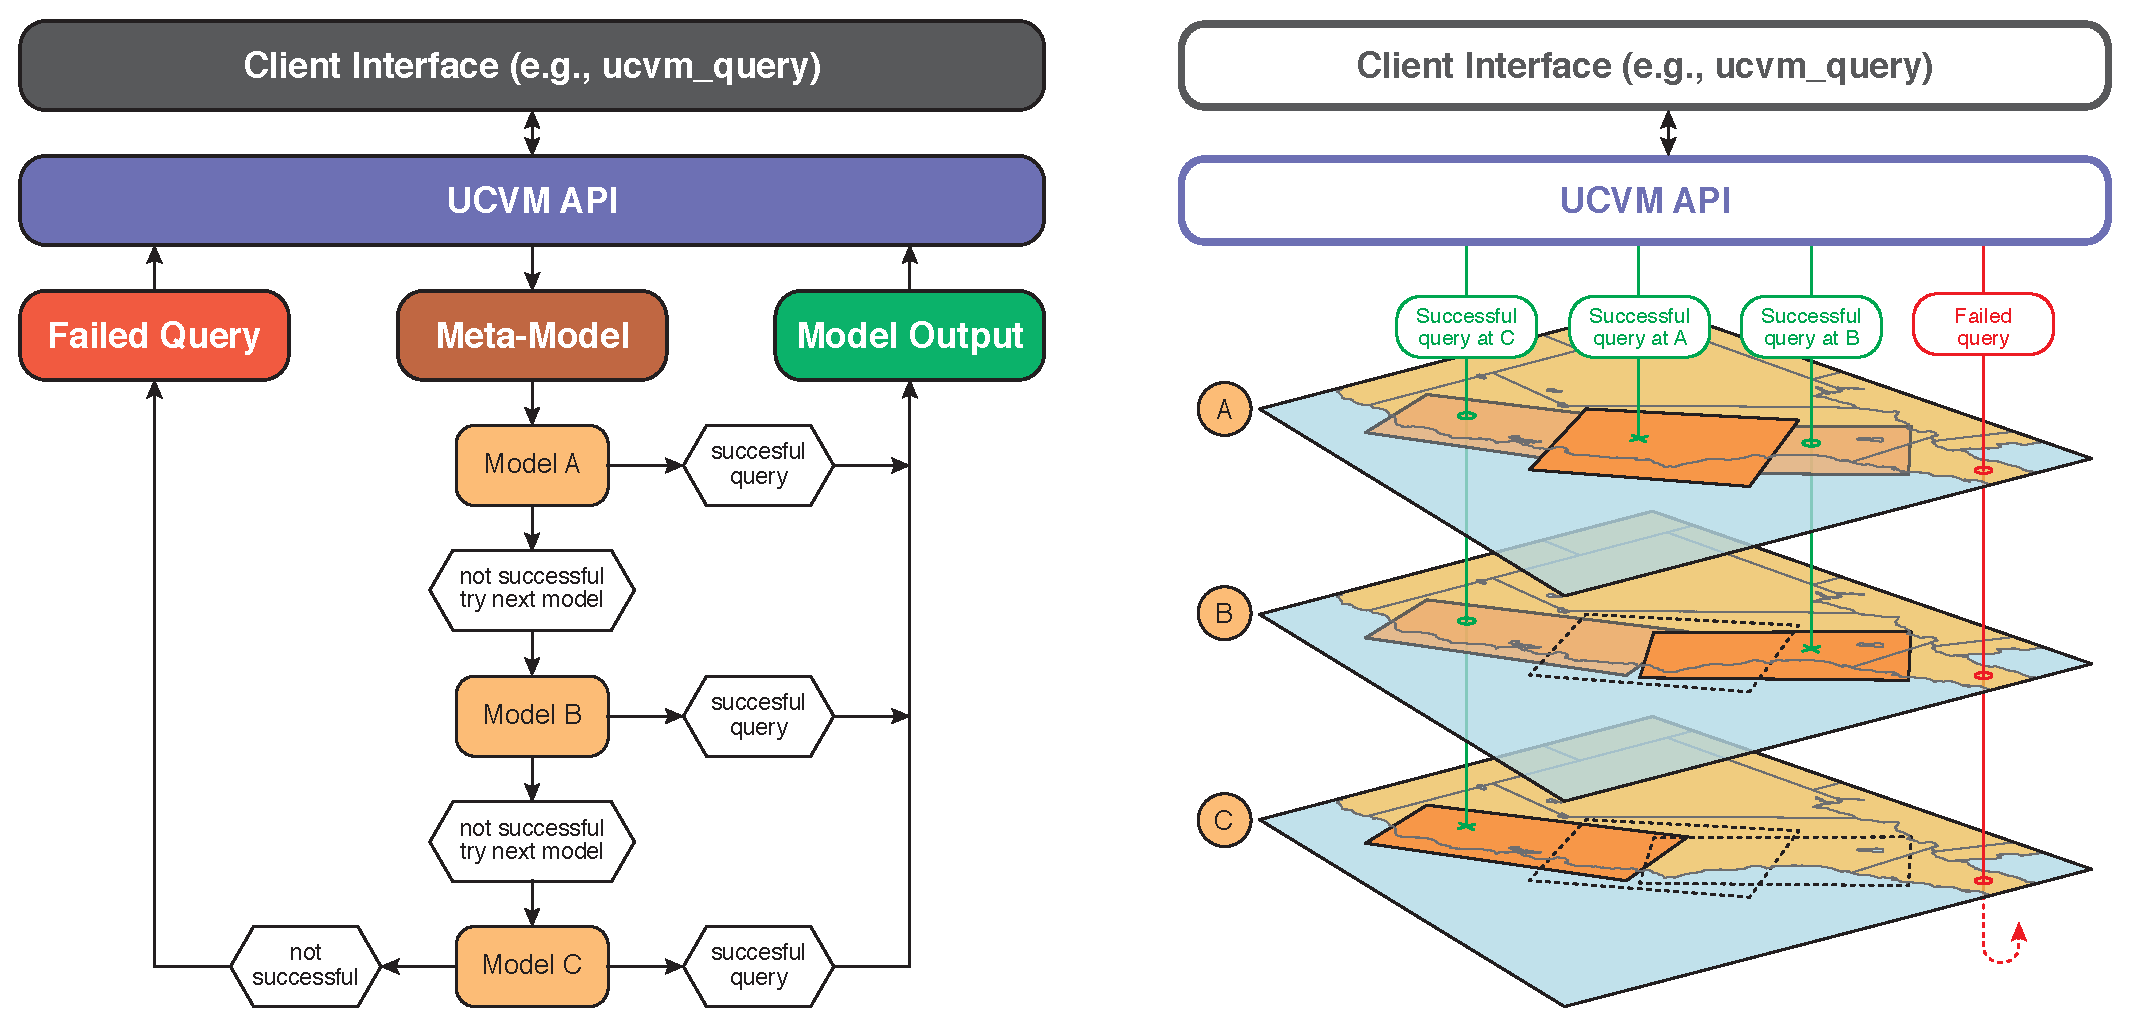
\includegraphics
		[width=0.75\textwidth]
		{figures/pdf/ucvm-query}
	\caption{UCVM querying scheme (left) and geographical illustration of the querying process (right). Information at a given geographic location is retrieved from the models registered in UCVM through a hierarchical querying scheme in which the user defines a preferred sequence of models, which are assembled internally in a meta-model. Queries to the models beneath the meta-model are carried out in the order specified by the user. Successful queried values (or failed-query results) are handled by the UCVM API wich is accessible to the user/client through a predefined interface such as the program \texttt{ucvm\_query}.}
	\label{fig:tiling}
\end{figure*}


\subsection{Querying Material Properties}
\label{sec:querying}

UCVM provides two methods for querying models. The first method is programmatically, directly through the provided C language API. The second is via the command-line program \texttt{ucvm\_query}. Both methods query the underlying models in the same manner; the \texttt{ucvm\_query} program is merely a simplified front-end layered upon the API.

The query process begins with the identification of one or more CVMs as the source of material properties. In this respect, the framework distinguishes between geotechnical layers and standard crustal models, allowing the user to make selections for both. As illustrated in Figure \ref{fig:tiling}, the set of standard crustal models is tiled in three dimensions to form a meta-model. The same operation is performed on the GTLs to define a meta-GTL. The interface between the meta-GTL and meta-model is then smoothed using an interpolation function (linear interpolation in the simplest case) along a user-defined interpolation zone parallel to the z-axis. Note that when two or more models overlap in three dimensional space, the model listed first within the tiling order will satisfy requests within that overlapping zone.

Once the models have been tiled in this manner, the API or program accepts one or more input query points from the user. For every point, the framework queries each component model of the two meta models, until either a valid set of velocities and density are returned, or all component models have been queried and the request was unsatisfied. Thus, for points that fall within the interpolation zone, two sets of material properties may be generated---one for each meta model. These two sets of material properties are then combined using the interpolation function. As the native query interfaces of available CVMs accept query points in a wide array of formats (e.g., geographic coordinates versus UTM-11 map coordinates, or depth versus elevation for the vertical component), UCVM may perform a coordinate transformation to convert its input format of decimal (latitude, longitude, depth/elevation) tuples to the local coordinate system of the component model being queried. This is accomplished transparently by utilizing the standard projection library Proj.4 \citep{Evenden_2003_Manual}.

In the case of the API, the result of a successful query is a data-structure containing the velocities \vp{} and \vs{}, and the density $\rho$ at the point of interest, along with the elevation in meters and $V_{S30}$ value of the corresponding point on the free-surface. This data-structure also includes an indicator of which velocity model within the meta-model ultimately satisfied the request. For those points which fall within the interpolation zone between the meta-GTL and meta-model, the framework additionally identifies the material properties reported by the meta-GTL and the meta-model, as well as the component models from which they were extracted. For the \texttt{ucvm\_query} program, this same information is formulated in tabular format and printed to the screen.

This tiling mechanism mostly allows one to complement missing information in one model with that of other overlapping or underlying models. In the future, the UCVM tiling feature could be used as tool for combining multiple regional velocity models. The platform, however, does not presently provide built-in functionalities to do so beyond the described tiling mechanism. The reason being that consistency problems arise when velocity models overlap in three-dimensional space. That is, tiling two overlapping models that are not compatible has the potential of creating interfaces with unnatural contrasts. These artifacts are undesirable for earthquake simulation applications because they can cause unexpected wave reflections or refractions. There are two approaches one can take to remedy this problem. The simplest approach is to define a UCVM patch model to trilinearly interpolate the material properties within a certain geographic region. This patch model may be tiled along with the overlapping traditional velocity models to produce a smoothed meta-model. However, this numerical smoothing approach may not reflect the physical structures of the Earth's surface. The second approach is to utilize UCVM to query all models within the overlap zone individually, and then manually combine the results with a user-defined interpolation function. We expect that future tomographic inversions of larger regions will allow us to integrate better models or algorithms to handle this situation.
